\section{Auswertung}

\subsection{Auswertung der Simulationsdaten}
Da die Simulationsdaten Events enthalten, welche für die Auswertung nicht relevant sind, werden diese zunächst selektiert. Die Verteilungen der Selektionsvariablen sind in Abbildung \ref{fig:Cuts_sim} abgebildet.
\begin{figure}
    \centering
    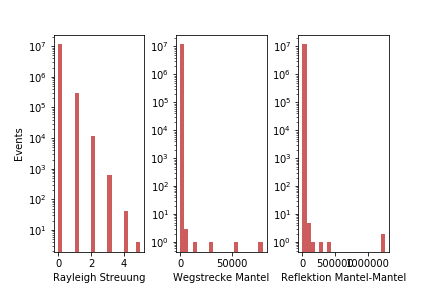
\includegraphics[width=0.5\textwidth]{plots/cuts_sim.pdf}
    \caption{Verteilung der Selektionsvariablen (von links nach rechts): Anzahl Rayleigh-Streuungen, Wegstrecke im Mantelmaterial, Reflektion an der Mantel-Mantel-Grenzfläche.}
    \label{fig:Cuts_sim}
  \end{figure}
  \FloatBarrier
Photonen, welche in der Faser gestreut werden, können nicht mehr durch die in Kapitel \ref{theorie} gefundenen Gleichungen beschrieben werden. Aus diesem Grund werden Ereignisse, deren Anzahl an Rayleigh-Streuungen (\textit{rayleighScatterings}) größer als Null ist, verworfen.
Des Weiteren soll im Folgenden zwischen Photonen unterschieden werden, welche sich lediglich im Kern bewegen und welche, die in den Mantel reflektiert werden. Die Ersten werden im Folgenden als Kernphotonen bezeichnet, während die Photonen, welche in den Mantel eindringen, Mantelphotonen genannt werden.
Zu den Mantelphotonen zählen die Photonen mit einer Wegstrecke im Mantelmaterial (\textit{length\_clad}) und einer Anzahl an Reflektionen an der Mantel-Mantel-Grenzfläche (\textit{reflClCl}) größer Null. \\

Im Anschluss wird für alle Photonen der Winkel $\theta$ zwischen der $x$-Achse der Faser und ihrer Wegstrecke bestimmt. Anhand von Abbildung \ref{fig:Geometrie} kann der Zusammenhang
\begin{align}
    \vec{p}\vec{e}_{\mathrm{x}} &= |\vec{p}||\vec{e}_{\mathrm{x}}| \cos(\theta) \\
    \Leftrightarrow \theta &= \arccos(p_{\mathrm{x}})
\end{align}
hergeleitet werden. Die Verteilung von $\theta$ für die Kern- und Mantelphotonen ist in Abbildung \ref{fig:theta_sim} dargestellt.
\begin{figure}
    \centering
    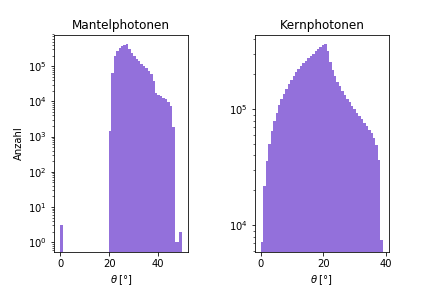
\includegraphics[width=0.5\textwidth]{plots/theta_sim.pdf}
    \caption{Verteilung vom Winkel $\theta$, welcher den Winkel des Photons zur $x$-Achse beschreibt, für die Kern- und Mantelphotonen.}
    \label{fig:theta_sim}
\end{figure}
\FloatBarrier
Die Kernphotonen weisen eine unsymmetrische Verteilung um etwa $\SI{20}{°}$ auf, wobei in dem Bereich oberhalb des Maximums weniger Photonen zu finden sind. Es werden Werte zwischen $\SI{0}{°}$ und $\SI{40}{°}$ angenommen. Die Verteilung der Mantelphotonen hingegen beginnt bei einem Winkel von etwa $\SI{20}{°}$ Grad und nimmt auch Werte etwas oberhalb von $\SI{40}{°}$ an.\\

Mit Hilfe der Histogramme wird das Verhältnis von Kern- und Mantelphotonen für jeden Winkel $\theta$ bestimmt, indem die Anzahl an Einträgen der Mantelphotonen pro Bin durch die Anzahl an Kernphotonen dividiert wird. In Abbildung \ref{fig:ratio_sim} sind die Verhältniswerte in Abhängigkeit von $\theta$ zu erkennen.
\begin{figure}
    \centering
    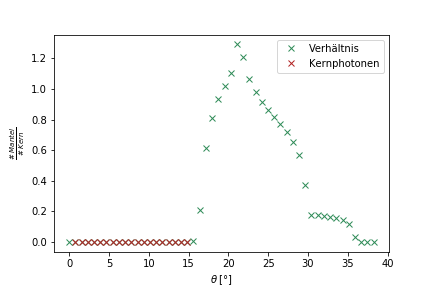
\includegraphics[width=0.5\textwidth]{plots/ratio_sim.pdf}
    \caption{Verhältnis von Kern- und Mantelphotonen in Abhängigkeit vom Winkel $\theta$ (grün). In rot sind die Winkelbereiche gekennzeichnet, in denen nur Kernphotonen auftreten.}
    \label{fig:ratio_sim}
\end{figure}
\FloatBarrier
Ein besonders starkes Vorkommen von Mantelphotonen ist in einem Winkelbereich von etwa $\SI{15}{°}$ bis $\SI{30}{°}$ zu erkennen, wobei sich das Maximum bei einem Winkel von etwas über $\SI{20}{°}$ befindet.

Verhältnisse von Kern- und Mantelphotonen mit dem Wert Null weisen auf Winkelbereiche hin, in denen lediglich Kernphotonen auftreten. Diese Bereiche sind in Abbildung \ref{fig:ratio_sim} mit der Farbe rot gekennzeichnet und treten für Winkelbereiche unterhalb von
\begin{align*}
    \theta_{\mathrm{nur Kern, max}} = \SI{14.82}{°}
\end{align*}
auf. \\

Der minimale Abstand $r_{\mathrm{min}}$ der Kernphotonen zur $x$-Achse kann über den Abstand windschiefer Geraden bestimmt werden. Hierzu wird der Weg des Photons mit der Gleichung
\begin{align}
    p(t) = \left(\begin{array}{c} x\_start \\ y\_start \\ z\_start \end{array}\right)
        + t \left(\begin{array}{c} px\_start \\ py\_start \\ pz\_start \end{array}\right)
\end{align}
und die $x$-Achse mit
\begin{align}
    a(s) = \left(\begin{array}{c} 0 \\ 0 \\ 0 \end{array}\right)
        + s \left(\begin{array}{c} 1 \\ 0 \\ 0 \end{array}\right)
\end{align}
parametrisiert.
Mit Hilfe des orthogonalen Vektors auf die Stützvektoren
\begin{align}
    \vec{n} = \vec{p}\; \times \; \vec{e}_{\mathrm{x}} = \left(\begin{array}{c} 0 \\ pz\_start \\ -py\_start \end{array}\right)
\end{align}
kann die Hilfebende
\begin{align}
    E = pz\_start \cdot y\_start - py\_start \cdot z\_start
\end{align}
konstruiert werden. Der Abstand ist dann schlussendlich durch
\begin{align}
    r_{\mathrm{min}} = \frac{|pz\_start \cdot y\_start - py\_start \cdot z\_start|}{\sqrt{pz\_start ^2 + py\_start^2}}
\end{align}
gegeben. Die Verteilung von $r_{\mathrm{min}}$ ist Abbildung \ref{fig:rmin_sim} zu entnehmen.
\begin{figure}
    \centering
    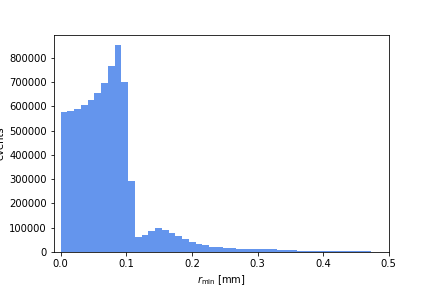
\includegraphics[width=0.5\textwidth]{plots/rmin_sim.pdf}
    \caption{Verteilung des minimalen Abstandes $r_{\mathrm{min}}$ zwischen Photonen und $x$-Achse.}
    \label{fig:rmin_sim}
\end{figure}
\FloatBarrier
Es lässt sich ein gleichmäßiger Anstieg der Verteilung bis zu einem Wert von $r_{\mathrm{min}} \approx \SI{0.1}{mm}$ erkennen, wo die Werte steil abfallen.
Anhand von $r_{\mathrm{min}}$ werden die Kernphotonen auf Daten zugeschnitten, deren $r_{\mathrm{min}}$ kleiner als der Radius der Kernfaser von $\SI{0.1}{mm}$ ist.\\

Zur Bestimmung des mittleren Abstandes pro Winkel werden die $r_{\mathrm{min}}$ in Abhängigkeit von $\theta$ in Abbildung \ref{fig:Hist_rmin_sim} in einem zweidimenesionalen Histogramm aufgetragen.
\begin{figure}
    \centering
    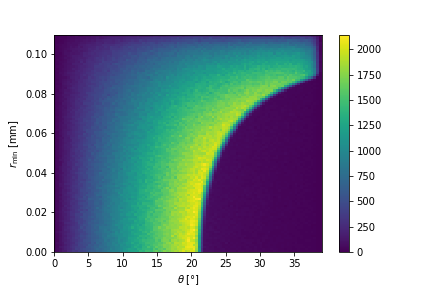
\includegraphics[width=0.5\textwidth]{plots/hist_rmin_sim.pdf}
    \caption{Zweidimenesionales Histogramm der $r_{\mathrm{min}}$ in Abhängigkeit von $\theta$.}
    \label{fig:Hist_rmin_sim}
\end{figure}
\FloatBarrier
Entlang der Achse eines jeden Winkels werden die $r_{\mathrm{min}}$-Werte, gewichtet mit den jeweiligen Einträgen der Histogramm-Matrix, addiert und durch die Summe der Histogramm-Matrixelemente dividiert. Die Mittelwerte von $r_{\mathrm{min}}$ in Abhängigkeit von $\theta$ sind in Abbildung \ref{fig:rmin_mean_sim} zu sehen.
\begin{figure}
    \centering
    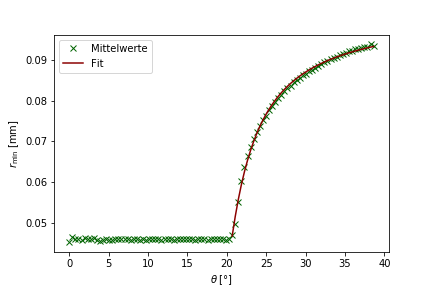
\includegraphics[width=0.5\textwidth]{plots/rmin_mean_sim.pdf}
    \caption{Mittelwerte der $r_{\mathrm{min}}$ in Abhängigkeit vom Winkel $\theta$. }
    \label{fig:rmin_mean_sim}
\end{figure}
\FloatBarrier
Die $r_{\mathrm{min}}$-Werte weisen bis zu einem Winkel von $\theta \approx \SI{20}{°}$ einen konstanten Wert von etwa $\SI{45}{\micro m}$ auf und steigen anschließend an.
In den Anstieg wird eine Fit-Funktion der Form
\begin{align}
    r_{\mathrm{min}}(\theta) = a \arctan(b + c \theta)
\end{align}
gelegt. Dieser Zusammenhang lässt sich durch Winkelrelationen in Abbildung \ref{fig:Geometrie} motivieren.
Mittels der Funktion \textit{curve\_fit} des Packetes \textit{scipy\_optimize} werden für die Parameter die Werte
\begin{align*}
    a &= (655 \pm 2)\cdot 10^{-4} ,\\
    b &= (-6.5 \pm 0.2),\\
    c &= (358 \pm 9)\cdot 10^{-3}
\end{align*}
ermittelt.

Aus Abbildung \ref{fig:Hist_rmin_sim} wird außerdem der maximale Winkel bestimmt, unter welchem Kernphotonen die Ausleseelektronik erreichen. In Abbildung \ref{fig:theta_max_grad_bsp} ist hierzu der winkelabhängige Verlauf der Photonenintensität beispielhaft für $r_\mathrm{min} = \SI{0.087}{mm}$, sowie der Gradient des Verlaufes dargestellt. Letzterer wird mit der Funktion \textit{numpy.gradient} berechnet. 
\begin{figure}
    \centering
    \includegraphics[width=0.5\textwidth]{plots/theta_max_grad_bsp.pdf}
    \caption{Oben: Verlauf der Photonenintensität in Abhängigkeit des Winkel $\theta$ für $r_\mathrm{min} = \SI{0.087}{mm}$. Unten: Gradient der Photonenintensität in Abhängigkeit des Winkel $\theta$ für $r_\mathrm{min} = \SI{0.087}{mm}$. }
    \label{fig:theta_max_grad_bsp}
\end{figure}
\FloatBarrier
Die Photonenintensität steigt stetig an und fällt anschließend steil auf etwa null ab. An der Stelle des Endpunktes dieses Abfalls ist ein Minimum des Gradienten erkennbar, da die Steigung ab diesem Punkt lediglich flach verläuft. Dieses Verfahren wird für alle $r_\mathrm{min}$-Werte durchgeführt.
Die Grenzwinkel $\theta_{\mathrm{max}}$ sind in Abbildung \ref{fig:theta_max_sim} gegen $r_{\mathrm{min}}$ aufgetragen.
\begin{figure}
    \centering
    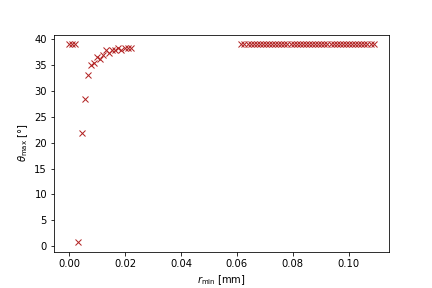
\includegraphics[width=0.5\textwidth]{plots/theta_max_sim.pdf}
    \caption{Grenzwinkel $\theta_{\mathrm{max}}$, unter welchem Photonen noch detektiert werden, in Abhängigkeit vom minimalen Abstand zur Faserlängsachse $r_{\mathrm{min}}$. }
    \label{fig:theta_max_sim}
\end{figure}
\FloatBarrier
Die Werte des maximalen Winkels steigen kontinuierlich zunächst langsam und zu höheren $r_{\mathrm{min}}$-Werten hin steiler an, bevor sie bei $r_\mathrm{min} \approx \SI{0.09}{mm}$ in eine Sättigung von $\theta_{\mathrm{max}}\approx \SI{38}{°}$ übergehen.


Des Weiteren werden die Reflektionswinkel $\theta_{\mathrm{refl}}$ nach Gleichung \eqref{eq:2} berechnet und ihre Verteilung in Abbildung \ref{fig:Theta_refl_sim} in Abhängigkeit vom Winkel $\theta$ aufgetragen.
\begin{figure}
    \centering
    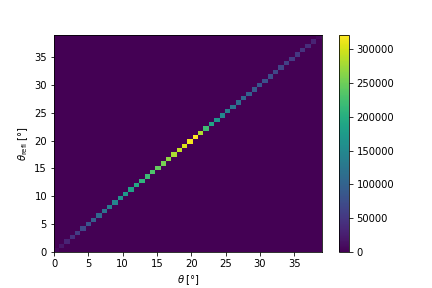
\includegraphics[width=0.5\textwidth]{plots/Theta_refl_sim.pdf}
    \caption{Verteilung der Reflektionswinkel $\theta_{\mathrm{refl}}$ in Abhängigkeit vom Winkel $\theta$. }
    \label{fig:Theta_refl_sim}
\end{figure}
\FloatBarrier
Analog zu den minimalen Abständen $r_{\mathrm{min}}$ werden die Mittelwerte des Reflektionswinkel pro Winkel $\theta$ bestimmt und in Abbildung \ref{fig:Theta_refl_mean_sim} in Abhängigkeit von $\theta$ dargestellt.
\begin{figure}
    \centering
    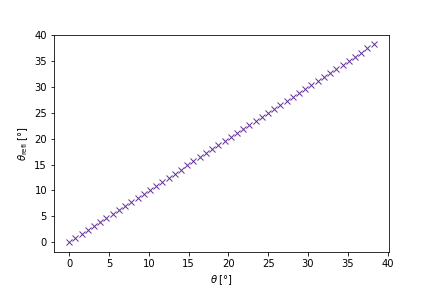
\includegraphics[width=0.5\textwidth]{plots/Theta_refl_mean_sim.pdf}
    \caption{Mittelwerte der Reflektionswinkel $\theta_{\mathrm{refl}}$ in Abhängigkeit vom Winkel $\theta$. }
    \label{fig:Theta_refl_mean_sim}
\end{figure}
\FloatBarrier
Es zeigt sich ein linearer Zusammenhang zwischen dem Reflektionswinkel $\theta_{\mathrm{refl}}$ und dem Winkel des Photons zur Faserachse $\theta$.

Für den Austrittswinkel $\alpha$ der Photonen, welcher über den horizontalen Winkel gemessen wird, kann über Winkelrelationen und das Snellius´sche Brechnungsgesetz der Zusammenhang
\begin{align}
    \alpha = \arcsin \left( \sin(\theta)\frac{n_\mathrm{K}}{n_\mathrm{Si}}\right)
\end{align} 
hergeleitet werden. Hierbei ist der Brechungsindex des Kernes durch $n_\mathrm{K} = 1.6$ \cite{anleitung} und des anschließenden Siliziums durch $n_\mathrm{Si} = 3.352$ \cite{si} gegeben.
Die Photonenintensität in Abhängigkeit vom Austrittswinkel ist in Abbildung \ref{fig:austritt_simu} für die Mantel- und Kernphotonen zu erkennen.
\begin{figure}
    \centering
    \includegraphics[width=0.5\textwidth]{plots/austritt_simu.pdf}
    \caption{Anzahl an Photonen als Funktion des Austrittswinkels $\alpha$ für die Mantel- (links) und Kernphotonen (rechts). }
    \label{fig:austritt_simu}
\end{figure}
\FloatBarrier

Zur Untersuchung der winkelabhängigen Abschwächung wird ein zweidimenesionales Histogramm erstellt, welches die Zählrate pro Ausfallwinkel $\alpha$ und Anregungsposition $x$ darstellt. Letzteres ist durch die Simulationsvariable \textit{gpsPosX} gegeben.
\begin{figure}
    \centering
    \includegraphics[width=0.5\textwidth]{plots/hist_x_alpha_simu.pdf}
    \caption{Zweidimensionales Histogramm der Photonenintensität in Abhängigkeit von dem Ausfallwinkel $\alpha$ und der Anregungsposition $x$. }
    \label{fig:hist_x_alpha_simu}
\end{figure}
\FloatBarrier
Die Abschwächung $a_\mathrm{eff}$ ist durch den Zusammenhang 
\begin{align}
    I(x) = I_{0} \exp(a_\mathrm{eff} \cdot x)
    \label{eq:exp_fit}
\end{align}
gegeben, mit der Photonenintensität $I(x)$ bei einer Anregung der Faser an der LED-Position $x$. 
Für jeden Winkel wird die Intensität, repräsentiert durch das jeweilige Element der Histogrammmatrix, in Abhängigkeit von $x$ aufgetragen und mittels der Funktion \textit{curve\_fit} des Packetes \textit{scipy\_optimize}  ein Fit von Gleichung \ref{eq:exp_fit} durchgeführt. Der Vorgang ist in Abbildung \ref{fig:fit_exp_simu_bsp} beispielhaft für den Winkel $\alpha = \SI{0}{°}$ dargestellt.
\begin{figure}
    \centering
    \includegraphics[width=0.5\textwidth]{plots/fit_exp_simu_bsp.pdf}
    \caption{Photonenintensität in Abhängigkeit von der Anregungsposition $x$, sowie die Fitfunktion zur Ermittlung der Abschwächung. Beispielhafte Abbildung für einen horizontalen Winkel von $\SI{0}{°}$.}
    \label{fig:fit_exp_simu_bsp}
\end{figure}
\FloatBarrier
Die Fitparameter $I_0$ und $a_\mathrm{eff}$ sind als Funktion des Austrittswinkels $\alpha$ in Abbildung \ref{fig:fit_exp_simu} zu erkennen.
\begin{figure}
    \begin{subfigure}[c]{0.5\textwidth}    
        \includegraphics[width=0.95\textwidth]{plots/fit_exp_simu.pdf}
        \subcaption{Abschwächung $a_\mathrm{eff}$.}    
    \end{subfigure}
    \begin{subfigure}[c]{0.5\textwidth}
        \includegraphics[width=0.95\textwidth]{plots/fit_exp_simu_I0.pdf}
        \subcaption{Anfangsintensität $I_0$.}
    \end{subfigure}
    \caption{Fitparameter $I_0$ und $a_\mathrm{eff}$ in Abhängigkeit des Austrittwinkels.}
    \label{fig:fit_exp_simu}
\end{figure}

\subsection{Auswertung der Messdaten}
Zur Überprüfung der Abdunklung des Versuchaufbaus werden die Photonenintensitäten der Untergrundsmessreihen ohne Faseranregung in Abbildung \ref{fig:Untergrund_Untersuchung} in Abhängigkeit von der Wellenlänge $\lambda$ aufgetragen.
\begin{figure}
    \centering
    \includegraphics[width=0.5\textwidth]{plots/Untergrund_Untersuchung.pdf}
    \caption{Photonenintensität durch Hintergrundbeleuchtung in Abhängigkeit von der Wellenlänge $\lambda$ für verschiedene Abdunklungsmaßnahmen.}
    \label{fig:Untergrund_Untersuchung}
\end{figure}
\FloatBarrier
Es lässt sich erkennen, dass für einen Aufbau mit abgedunkelten Raum und abgedecktem Versuchsaufbau der Hintergrund deutlich minimiert werden kann. Dieser Aufbau wird für die weiteren Messungen verwendet. 
Im Vergleich der beiden Winkeleinstellungen lässt sich erkennen, dass die Abschirmung des Hintergrundes nicht für alle Winkel gleich gut funktioniert. 
Für eine weitere Reduzierung des Einflusses der Hintergrundsbeleuchtung wird daher in jeder Messposition der Dunkelstrom aufgenommen und von den gemessenen Photonenintensitäten subtrahiert.

Zur Überprüfung der Radialsymmetrie werden die aufgenommenen Zählraten nach Abziehen des Dunkelstroms für alle Wellenlängen, sowie für jeweils jeden horizontalen und jeden vertikalen Winkel aufsummiert. Die winkelabhängigen Counts sind in Abbildung \ref{fig:radial_test} zu erkennen. 
\begin{figure}
    \centering
    \includegraphics[width=0.5\textwidth]{plots/radial_test.pdf}
    \caption{Aufgenommene Zählrate in Abhängigkeit vom horizontalen Winkel (links) und vertikalen Winkel (rechts) zur Überprüfung der Radialsymmetrie.}
    \label{fig:radial_test}
\end{figure}
\FloatBarrier
Beide Verteilungen lassen eine Radialsymmetrie erahnen, wobei der Mittelpunkt, welcher sich durch eine maximale Photonenintensität auszeichnet, leicht vom Winkel Null verschoben ist. Für die folgenden Auswertungsschritte wird von einer radialsymmetrischen Verteilung ausgegangen.


Zur Untersuchung der Abschwächung der Photonenintensität entlang der Faser wird zunächst der relevante Wellenlängenbereich ermittelt. Dazu wird die Zählrate in Abhängigkeit von der Wellenlänge beispielhaft für die LED-Position $x = \SI{0}{cm}$ und einen horizontalen Winkel von $\SI{-10}{°}$ aufgetragen. Die gewählten Schnittgrenzen sind in Abbildung \ref{fig:wellenlaengen_cut} durch die gestrichelte Linie gekennzeichnet.
\begin{figure}
    \centering
    \includegraphics[width=0.5\textwidth]{plots/wellenlaengen_cut.pdf}
    \caption{Verteilung der wellenlängenabhängigen Photonenintensität für eine LED-Position von $x = \SI{0}{cm}$ und einem horizontalen Winkel von $\SI{-10}{°}$. In dunkelgrün sind die Schnittgrenzen zur Auswahl des relevanten Wellenlängenbereiches zu erkennen.}
    \label{fig:wellenlaengen_cut}
\end{figure}
\FloatBarrier
Im Folgenden werden Daten aus dem Wellenlängenbereich $\SI{420}{nm} \leq \lambda \leq \SI{640}{nm}$ verwendet.

Zur Berechnung der Abschwächung wird analog zur Auswertung der Simulationsdaten ein Fit der Gleichung \eqref{eq:exp_fit} für jede Wellenlänge und jeden Winkel durchgeführt. Die gefitteten Messpunkte sowie die Fitfunktion sind in Abbildung \ref{fig:Fit_exp_bsp} beispielhaft für eine Wellenlänge von $\lambda = \SI{440.589}{nm}$ und einen horizontalen Winkel von $\SI{-10}{°}$ zu erkennen.
\begin{figure}
    \centering
    \includegraphics[width=0.5\textwidth]{plots/Fit_exp_bsp.pdf}
    \caption{Messpunkte der Photonenintensität in Abhängigkeit von der LED-Position $x$, sowie die Fitfunktion zur Ermittlung der Abschwächung. Beispielhafte Abbildung für eine Wellenlänge von $\lambda = \SI{440.589}{nm}$ und einen horizontalen Winkel von $\SI{-10}{°}$.}
    \label{fig:Fit_exp_bsp}
\end{figure}
\FloatBarrier
Die Fitparameter $I_0$ und $a_\mathrm{eff}$ werden im Anschluss über die Wellenlängen gemittelt und in Abbildung \ref{fig:a_I0_winkel} als Funktion des horizontalen Winkels dargestellt. Der Fehler ergibt sich durch eine Mittelung des Fehlers der Fitparameter.
\begin{figure}
    \begin{subfigure}[c]{0.5\textwidth}    
        \includegraphics[width=0.95\textwidth]{plots/Abschwaechung_winkel.pdf}
        \subcaption{Abschwächung $a_\mathrm{eff}$.}    
    \end{subfigure}
    \begin{subfigure}[c]{0.5\textwidth}
        \includegraphics[width=0.95\textwidth]{plots/I0_winkel.pdf}
        \subcaption{Anfangsintensität $I_0$.}
    \end{subfigure}
    \caption{Fitparameter $I_0$ und $a_\mathrm{eff}$ in Abhängigkeit des horizontalen Winkels.}
    \label{fig:a_I0_winkel}
\end{figure}

Für die Ermittlung des wellenlängenabhängigen Reflektionskoeffizienten $\epsilon$ wird ein Fit von Gleichung \eqref{eq:9} durchgeführt. Hierzu wird aus dem horizontalen Winkel $\alpha$ der Winkel des Photons zur Faserachse $\theta$ mittels 
\begin{equation}
    \theta = \arcsin \left( \sin(\alpha)\frac{n_\mathrm{Si}}{n_\mathrm{K}}\right)
    \label{eq:theta}
\end{equation}
berechnet. Da die Winkel zur Faserachse $\theta$ relativ sind und keine negativen Werte annehmen, wird der Betrag der Winkelwerte ermittelt. Verwendet werden für den Fit lediglich Kernphotonen, da nur diese durch die im Theorieteil dargestellten Formeln beschrieben werden können. Aus Abbildung \ref{fig:austritt_simu} kann als Grenzwinkel ein horizontaler Winkel von $\alpha \approx \SI{15}{°}$ abgelesen werden.
Für den minimalen Abstand zur Faserachse kann aus Abbildung \ref{fig:rmin_mean_sim} für die verwendeten Winkel ein Mittelwert von $r_\mathrm{min} = \SI{0.06}{mm}$ bestimmt werden, während der Kernradius durch $r_\mathrm{Kern} = \SI{0.11}{mm}$ \cite{anleitung} gegeben ist.
Zur Durchführung des Fits wird nun für jede Wellenlänge die Abschwächung $a_\mathrm{eff}$ in Abhängigkeit vom Winkel $\theta$ aufgetragen und nach Gleichung \eqref{eq:9} gefittet. Dieses ist in Abbildung \ref{fig:fit_a_bsp} beispielhaft für eine Wellenlänge von $\lambda = \SI{440.589}{nm}$ dargestellt.
\begin{figure}
    \centering
    \includegraphics[width=0.5\textwidth]{plots/fit_a_bsp.pdf}
    \caption{Beispielhafte Darstellung des Fits von der Abschwächung $a_\mathrm{eff}$ als Funktion des Winkel $\theta$ zur Ermittlung des Reflektionskoeffizienten $\epsilon$ für $\lambda = \SI{440.589}{nm}$.}
    \label{fig:fit_a_bsp}
\end{figure}
\FloatBarrier
Die Fitparameter $a_0$ und $\epsilon$ sind in Abbildung \ref{fig:a0_epsilon} in Abhängigkeit von der Wellenlänge aufgetragen.
\begin{figure}
    \begin{subfigure}[c]{0.5\textwidth}    
        \includegraphics[width=0.95\textwidth]{plots/a0_lamda.pdf}
        \subcaption{Parameter $a_0$.}    
    \end{subfigure}
    \begin{subfigure}[c]{0.5\textwidth}
        \includegraphics[width=0.95\textwidth]{plots/reflektionskoeff_lamda.pdf}
        \subcaption{Reflektionskoeffizient $\epsilon$.}
    \end{subfigure}
    \caption{Fitparameter $a_0$ und $\epsilon$ als Funktion der Wellenlänge $\lambda$.}
    \label{fig:a0_epsilon}
\end{figure}
\FloatBarrier

Durch Umstellen von Gleichung \eqref{eq:9} nach $\epsilon$ kann für den Reflektionskoeffizienten als Funktion des Winkels $\theta$ der Zusammenhang 
\begin{align}
    \epsilon = \frac{2\sqrt{r_\mathrm{Kern}^2 -r_\mathrm{min}^2 }}{\tan(\theta)} \left(a_\mathrm{eff}-\frac{a_0}{\cos(\theta)}\right)
    \label{eq:eps}
\end{align}
bestimmt werden. Bei der Berechnung von $\theta$ nach Gleichung \eqref{eq:theta} liefern nicht alle vermessenen Winkel einen zulässigen Wert für $\theta$: Für Austrittswinkel oberhalb von $\SI{20}{°}$ ist Formel \eqref{eq:theta} nicht gültig. 
Für den zulässigen Bereich wird demnach der winkelabhängige Reflektionskoeffizient nach \eqref{eq:eps} berechnet und in Abbildung \ref{fig:reflektionskoeff_winkel} dargestellt. Für einen Winkel von $\theta = \SI{0}{°}$ ergibt sich durch die Division mit Null ein Wert von Unendlich, weshalb dieser ebenfalls vernachlässigt wird. Der Fehler wird mittels der Gauß´schen Fehlerfortpflanzung von $a_\mathrm{eff}$ und $a_\mathrm{0}$ ermittelt.
\begin{figure}
    \centering
    \includegraphics[width=0.5\textwidth]{plots/reflektionskoeff_winkel.pdf}
    \caption{Reflektionskoeffizient $\epsilon$ als Funktion des Winkels zur Faserachse $\theta$. Die Unsicherheiten überdecken einen Teil der Werte.}
    \label{fig:reflektionskoeff_winkel}
\end{figure}
\FloatBarrier